\section{Durchf\"uhrung}

\begin{wrapfigure}{r}{.5\linewidth}
    \centering
    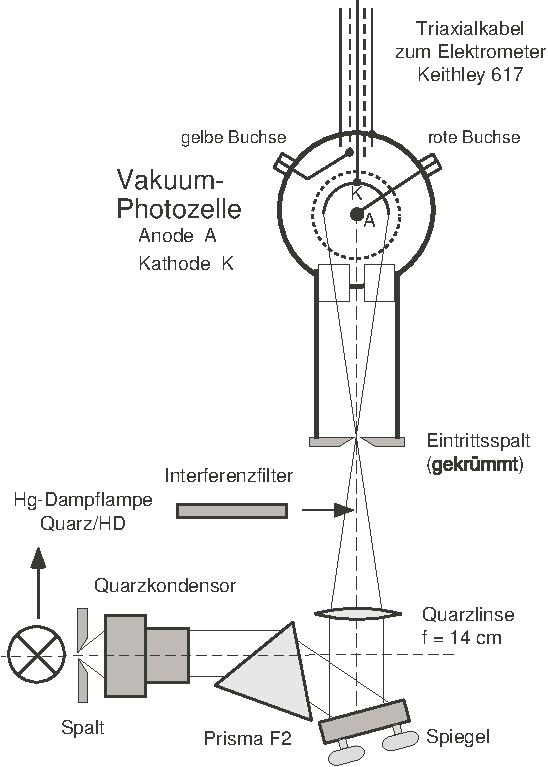
\includegraphics[width=\linewidth]{images/aufbau.pdf}
    \caption{Versuchsaufbau}
\end{wrapfigure}

Das Licht  einer  Hg-Damp-Lampe wird mit Hilfe eines Flint-Prismas F2 spektral
zerlegt und f\"allt \"uber einen Oberfl\"achenspiegel auf  den  Eintrittsspalt
der  Photozelle.  Die Anode ist durch  eine  Blende  abgeschattet.  Wegen  der
unterschiedlichen Lichtwege  im Prisma ist das Spaltbild leicht gekr\"ummt. Es
wird   durch  Verschieben  der  Quarzlinse  scharf  gestellt   und   mit   den
Stellschrauben des Spiegels justiert.  Die  Spaltbreite  ist  so einzustellen,
dass die  Hg-Linien  gelb  und  gr\"un  gerade  deutlich  getrennt  sind.  Vor
Messbeginn muss  man  die  HG-Dampf-Lampe  etwa 10 Min. einbrennen lassen. Zur
Absorption von  UV-Licht  wird  f\"ur alle $\lambda > 400$ \SI{}{\nano\meter} das
Langpassfilter Schott OG 400 zwischen Kondensor und Prisma geschaltet. Bei der
gr\"unen  und  gelben Hg-Linie wird kurzwelligeres  Streulicht  ebenfalls  mit
Hilfe von Kantenfiltern eliminiert.

Elektronen  in  der  Photokathode  absorbieren  die  Energie  $h\cdot\nu$  der
einfallenden Photonen. Ist ihre Energie anschliessend hoch  genug, so k\"onnen
sie das Metall  verlassen  und  fuhren  so  zu  einer  positiven Aufladung der
beleuchteten Elektrode. Die Elektronen haben nach  dem  Verlassen  der Kathode
eine  gewisse  maximale  kinetische Energie $E_{kin}$, die aber nicht ganz der
Energie  der absorbierten Photonen entspricht, sondern  etwas  niedriger  ist.
Dies  liegt  daran,  dass  beim  Austritt  aus  jedem Material die  sogenannte
Austrittsarbeit  $W_A$ aufgebracht werden muss, bzw. beim Eintritt wieder frei
wird. Es gilt die Gleichung:

\begin{equation}
    E_{kin} = \frac{1}{2}m_e v^2 = h\cdot\nu - W_{A,Kathode}
\end{equation}

\begin{wrapfigure}{r}{.5\linewidth}
    \centering
    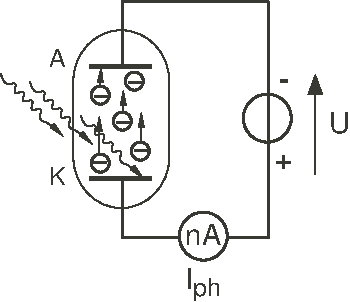
\includegraphics[width=\linewidth]{images/millikan.pdf}
    \caption{Messaufbau zur Messung der Gegenspannung}
    \label{fig:millikan}
\end{wrapfigure}

Die  Messung  der  maximalen  kinetischen  Energie  der  Elektronen  kann  auf
verschiedene   Arten   erfolgen.   Denkbar    w\"are    zum    Beispiel    die
Fluggeschwindigkeit  direkt  zu  bestimmen.  Allerdings  w\"are   ein  daf\"ur
geeigneter Aufbau  sehr  aufw\"andig.  Einfacher  ist es, zwischen Kathode und
Anode  eine Gegenspannung anzulegen, die gerade so eingestellt wird, dass auch
die  schnellsten  Elektronen  die  Anode  gerade  nicht  mehr  erreichen.  Der
(relativ) einfach  messbare  Photostrom  wird  fur  diesen Wert $U_{max}$ dann
gerade  null.  $U_{max}\cdot e$ entspricht bis auf einen konstanten  Summanden
der kinetischen Energie $E_{kin}$. Die Konstante kommt daher, dass nat\"urlich
nicht nur die Kathode, sondern auch die Anode eine Austrittsarbeit hat. Da die
beiden  Elektroden  \"uber  das Messger\"at verbunden sind, muss auch noch die
Kontaktspannung   berucksichtigt   werden,   so    dass   schliesslich   gilt:

\begin{align}
    U_{max}(\nu)\cdot e &= E_{kin} - U_{Kontakt} \cdot e \\
                        &= \left(h\cdot\nu - W_{A,Kathode}\right) - \left(W_{A,Anode}-W_{A,Kathode}\right) \\
                        &= h\cdot\nu - W_{A,Anode}
    \label{eq:umax}
\end{align}

Die Austrittsarbeit der Kathode spielt f\"ur den Wert  der  Gegenspannung also
tats\"achlich keine Rolle. Ihre Gr\"osse entscheidet aber nat\"urlich trotzdem
dar\"uber,  ob  \"uberhaupt  Photoelektronen emittiert werden k\"onnen und wie
hoch  deren kinetische Energie ist. Die Austrittsarbeiten h\"angen  nicht  von
der  Frequenz  des  eingestrahlten Lichtes ab. Deshalb kann man auch ohne ihre
Kenntnis  mit  Hilfe  der  Gleichung  \ref{eq:umax}  aus  zwei  Messungen  von
$U_max(\nu)$  f\"ur  verschiedene  Lichtfrequenzen  $\nu_1$  und $\nu_2$ durch
Differenzbildung die Konstante $h$ bestimmen:

\begin{equation}
    h = \frac{e\cdot\left(U_{max}(\nu_2) - U_{max}(\nu_1)\right)}{\nu_2 - \nu_1}
\end{equation}

Oder, falls mehrere Messdaten vorhanden sind, kann mittels linearer Regression
die Konstante $h$ auch anhand der Steigung berechnet werden:

\begin{equation}
    h = e \cdot m
    \label{eq:h}
\end{equation}

Wobei $m$ die Steigung des Fits der Funktion  $U_{max}(\nu)  =  m\cdot\nu + q$
ist.

Die  Tatsache,  dass  zwar  die  Anzahl, jedoch (zumindest fur  konventionelle
Lichtquellen)   nicht   die   Energie  der  austretenden  Elektronen  von  der
Intensit\"at  der   Strahlung   abh\"angt,   f\"uhrte   um   1900  zu  grossen
Erkl\"arungsschwierigkeiten im Rahmen der allgemein akzeptierten Wellentheorie
des Lichtes. Die Beobachtung, dass die Farbe, und damit die Wellenl\"ange bzw.
Frequenz, die Energie der Elektronen bestimmte, war v\"ollig unverst\"andlich.
Die Probleme konnten erst durch die im Jahr 1905 von  Einstein  vorgeschlagene
quantenmechanische Deutung des Photoeffektes beseitigt werden.

Bei der Photozelle handelt es sich um eine Vakuum-Photodiode CETRON  1P39. Die
Photokathode  hat  die   Form   eines  Halbzylinders,  ihre  Oberfl\"ache  ist
unbekannt. Die Anode ist als axialer Stift  ausgebildet  und durch eine Blende
abgeschattet.  Diese  Geometrie ist nicht gerade g\"unstig und hat  zur  Folge
dass  der  Photostrom nicht scharf einsetzt, d.h. die Dioden-Kennlinie  keinen
guten  ``Knick''  aufweist.  Aus  diesem  Grund  kann  man  nicht einfach  die
Kennlinie  aufnehmen,  sondern muss den Einsatzpunkt ``von Hand'' suchen.  Die
Zelle  ist  mit  einem  Triaxialkabel  an   das   Keithley   Elektrometer  617
angeschlossen.  Der  Zentralleiter ist mit der  Kathode  verbunden,  w\"ahrend
Anode  und  innerer  Schirm  separat  auf Buchsen  herausgef\"uhrt  sind,  die
\"aussere Abschirmung ist geerdet.

